\chapter{Hardware}
\label{chap:hardware}

This chapter presents the general architectures of a CPU and a GPU.
Furthermore, we present Amdahl's Law and Gustafson-Barsis Law, which discuss two different aspects of parallel execution compared to sequential execution.
We end the chapter by discussing why it is not a good idea to go all in with the GPU and no longer use a CPU.

First, we present \cref{tab:hardware connections transfer rates} which summarises the transfer rates of different connections of the different types of hardware.
We add \cref{fig:cpu gpu communication} to illustrate the connections these have.\todo{add table and figure}

\section{General Multi-core CPU Architecture}
\label{sec:cpu}

We will consider the architecture of a general multi-core Central Processing Unit (CPU) and what memory it can communicate with.
A multi-core CPU has two or more independent processing cores, which are Multiple Instructions Multiple Data (MIMD) cores.
This means that they can work on different instructions with different data simultaneously.

These cores have at least one layer of private cached memory.
Furthermore, there is at least one layer of public memory, where the largest is called Random Access Memory (RAM), and it thus shared memory between all the cores.
The further down the layered hierarchy the given memory is, the slower it is for the CPU to receive data from it.

\section{General GPU Architecture}
\label{sec:gpu}

The Graphical Processing Unit (GPU) is a device which is attached to a host machine.
This means that the GPU is an attached piece of hardware, which then is a work horse that works together with the CPU to perform computations.
We present \cref{fig:sm example} as a reference for this section.

\begin{figure}[htb]
  \centering
  \includegraphics[width=.5\textwidth]{graphics/images/cropped-cuda-sm.png}
  \caption{Example of a Streaming Multiprocessor for reference~\cite{farber2011cuda}}
  \label{fig:sm example}
\end{figure}

A GPU's basic building block is the streaming multiprocessor (SM), which is independently responsible for its own resources, cores, and memory.
By making each SM independent memory access and computation are performed faster, because there is not global memory or special units that are shared among all the hardware.
Each SM has Single Instruction Multiple Data (SIMD) Arithmetic Logic Units (ALU), which are commonly referred to as the cores.
These cores will all run the same instruction, but may use different data.

The work given to the GPU is distributed to the SMs by the Giga-Thread global scheduler, which knows when the SMs are busy.
CUDA-enabled devices are categorised by their compute capability which describes the amount of threads each block can have.
Threads actually perform computations.
They are organised into blocks and grids.
These are described further in \cref{chap:software}.

The SMs receive instructions in a cache and warp schedulers distribute the work to the cores, so the instructions can be executed.
Each thread has access to its own registers, which is called its local memory.
Each SM has shared memory for high-speed data sharing between threads in a block.
The GPU as a whole has memory called global memory, which is accessible by all the GPU's SMs.

Furthermore, an SM has load/store (LD/ST) units and Special Function Units (SFU).
LD/STs calculate source and destination addresses and loads/store data as needed.
SFUs execute special functions, e.g. sin, sqrt, etc.
Each SFU executes one instruction per thread per clock.
SFUs can perform an operation while it is communicating with another thread.
Compared to the SIMD cores, the SFUs are designed specifically to perform their designated functions, and the SIMD cores are general purpose cores.

% good warp answers:  http://stackoverflow.com/questions/11816786/why-bother-to-know-about-cuda-warps
%                     http://stackoverflow.com/questions/10460742/how-do-cuda-blocks-warps-threads-map-onto-cuda-cores
A warp is a block of 32 SIMD threads, and they are the basic unit for scheduling work in the SMs.
To maximize the utilisation of the GPU the developer must make sure that these warp sizes are considered when executing code.
If one does not consider the warp size and randomly schedules tasks, then the programs might have many idle threads that do nothing.
If this is the case, then the GPU is not utilised to its optimal capacity~\cite{fermi2009nvidia}.

\subsection{Hardware Specific Numbers}
\label{sec:hardware specific numbers}

Throughout this report, we will be using the Tesla K40 GPU~\cite{teslak402013nvidia}.
For future reference \cref{tab:tesla k40 specs} presents the specifications for our GPU device.
In \cref{ap:tesla k40 specifications} we walk through how we found the specifications for our device.
\todo{is L1 cache used for shared memory?}

\begin{table}[htb]
  \centering
  \begin{tabular}{l r}
    \toprule
    item                        & limit \\
    \midrule
    warp size                   & \SI{32}{} \\
    max threads / block         & \SI{1024}{} \\
    total cores                 & \SI{2880}{} \\
    registers / block           & \SI{65536}{} \\
    constant memory             & \SI{65536}{B} \\
    L1 cache / block            & \SI{49152}{B}  \\
    L2 cache / core             & \SI{1572864}{B}  \\
    global memory               & \SI{12079136768}{B} \\
    \bottomrule
  \end{tabular}
  \caption{Tesla K40 GPU's specifications}
  \label{tab:tesla k40 specs}
\end{table}

Furthermore, the maximum dimension of grids and blocks are presented in \cref{tab:tesla k40 grid and block}.

\begin{table}[htb]
  \centering
  \begin{tabular}{r r r r}
    \toprule
    item & x & y & z \\
    \midrule
    block size & \SI{1024}{} & \SI{1024}{} & \SI{64}{} \\
    grid size  & \SI{2147483647}{} & \SI{65535}{} & \SI{65535}{} \\
    \bottomrule
  \end{tabular}
  \caption{Tesla K40 GPU's block and grid sizes}
  \label{tab:tesla k40 grid and block}
\end{table}

\section{Parallel Performance}
\label{sec:parallel performance}

This section presents two laws that aim to describe two different things when discussing performance speedup.
The first is Amdahl's Law which describes how much faster a program can become with the same workload, and the second is Gustafson-Barsis Law which describes how much more work can be performed with the same running time.
However, neither take into account that all computations have some overhead, e.g. reading and writing data, atomic operations where threads wait for each other, creating or deleting threads, etc.

\subsection{Amdahl's Law}
\label{sec:amdahls law}

Amdahl's Law is an equation that aims to approximate the potential speedup of a serial program.
The equation is presented in \cref{eq:amdahls law}, where $P$ is the portion of the serial code that can be parallelized, $(1-P)$ is the portion that cannot be made parallel, and we have $n$ processors.
Thus, $S(n)$ approximates the speedup by making a program parallel.

\begin{equation}
  \label{eq:amdahls law}
  S(n) = \frac{1}{(1-P) + P/n}
\end{equation}

Amdahl's Law only applies if the amount of work performed in the parallel version is not significantly different than the serial code's amount of work.
An illustration of the potential speedup is presented in \cref{fig:amdahls law} with $n=1024$.
It shows that the optimal solution is that the entire portion of code can be made parallel, and the code runs $n$ times faster compared to the serial code, when running $n$ processors~\cite{farber2011cuda}.

\begin{figure}[htb]
  \centering
  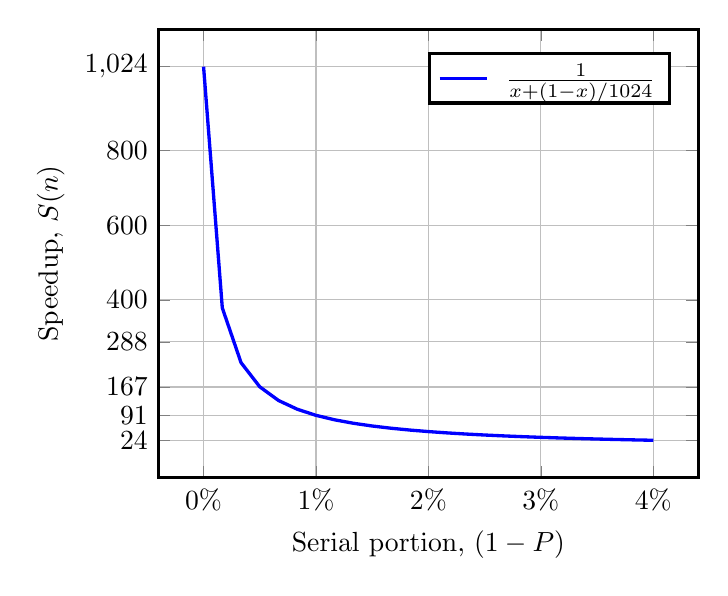
\begin{tikzpicture}
  \begin{axis}[
    ymajorgrids,
    xmajorgrids,
    ylabel={Speedup, $S(n)$},
    ytick={24,91,167,288,400,600,800,1024},
    xlabel={Serial portion, $(1-P)$},
    scaled x ticks = false, % do not add axis-multiplier
    xticklabel={% print percent
      \pgfmathparse{\tick*100}%
      \pgfmathprintnumber{\pgfmathresult}%
      \%%
    },
    legend style={
      at={(0.95,0.95)},
      anchor=north east,
      column sep=1ex
     },
     no markers,
     very thick
  ]

  \addplot+[domain=0.00:0.04] {1/(x+((1-x)/1024))};
  \addlegendentry{$\frac{1}{x + (1-x) / 1024}$};
  \end{axis}
\end{tikzpicture}

  \caption{Speedup given by Amdahl's Law with variable portions of paralleliable code $P$ and $n=1024$ processors}
  \label{fig:amdahls law}
\end{figure}

Notice how steep the curve is when having a portion of the code that is not parallelizable of 1\% to 0\%.
With 1\% serial portion the speedup is about $91\times$, and $1024\times$ when everything can be made parallel.
So, with just a tiny portion of the code that can only be serial, a high speedup is not likely to be achieved.

\subsection{Gustafson-Barsis Law}
\label{sec:gustafson-barsis law}

Gustafson-Barsis Law aims to overcome the shortcomings of Amdahl's Law, which says that the size of the problem is unchanged when made parallel.
The point that Gustafson makes is that many computational problems scale with the number of processors available, e.g. computing pi -- if we have more computational power, we compute more digits of pi~\cite{amdahlorgustafson2011}.
Note, however that if the goal at hand is to compute pi quicker, then that is ofcourse possible, this is just not what Gustafson-Barsis Law aims to describe.

\begin{equation}
  \label{eq:gustafson-barsis law}
  W(n) = n + (1-n) \times (1-P)
\end{equation}

So, the goal is to run a program in the same amount of time but with more work.
This approximation is present in \cref{eq:gustafson-barsis law}.
Thus, $W(n)$ gives the amount of work that can be further performed~\cite{gustafson1988reevaluating}.


% cpu vs. gpu: http://superuser.com/questions/308771/why-are-we-still-using-cpus-instead-of-gpus
\section{Do we ditch the CPU, and keep the GPU?}
\label{sec:cpu vs gpu}

It is true that a GPU has many more cores than a CPU, but these cores are significantly slower than the ones in a CPU.
These two processing units are developed with two different goals, and thus have different characteristics.

In general a CPU is a multi-purpose processing unit, whereas the GPU is a single-purpose compute-intensive processing unit.
The GPU has many more cores than the CPU, but the CPU's cores are much faster.
The memory hierarchy of a GPU enables it to efficiently compute instructions in parallel.
The CPU excels at sequential problems, that are not easily made parallel, because it is much faster.

Furthermore, GPUs do not have the features, e.g. interrupts and virtual memory, for modern operating systems.
One must consider a GPU as a compute-intensive problem solver, and nothing else.

